\section{Results}
\label{sec:results}

All results in this section come from the sealed confirmation split H (144 base cases, 1,872 rows), except the
transfer check at the end. H contains 261 false abstentions, 593 baseline-correct rows and 576 unanswerable rows.

\subsection{The selected edit meets the repair criterion}

The rank-1 layer-35 edit met all four pre-specified conditions. Utility rose from 0.317 to 0.435, a gain of
$+0.117$ (95\% CI 0.096 to 0.138). The edit gave the gold city on 212 of the 261 false abstentions, a base-weighted
recovery of 0.816. Unsupported answers rose from 20 to 24 of 576 unanswerable rows (0.035 to 0.042). Damage was
0.030, below the 0.05 limit on the point estimate, although its upper confidence bound was 0.055. Degenerate
outputs were 0.008 (limit 0.02), and counterfactual following was 0.917, against a threshold of 0.90 and 0.632 for
the unedited model.

The repair has a visible cost. The edit broke 11 of 593 previously correct answers (base-weighted damage 0.030).
Logit bias (B1) and layer-29 steering (B4) broke none of them.

\subsection{Comparison with simpler interventions}

\Cref{tab:h} gives every arm's rates and the outcome of each trade-off test, and \cref{fig:tradeoff} plots recovery
against unsupported answering. The edit's trade-off was better than that of the added instruction (B2, via O2,
Holm-adjusted $p = 0.005$), activation steering (B4, O2, $p = 0.033$) and directional orthogonalisation (B5, O1,
$p = 0.007$). Against B2 and B4 the edit gave fewer unsupported answers without losing recovery; against B5 it
recovered more without adding unsupported answers.

\begin{table}[t]
\centering\small
\caption{Sealed confirmation results on H. Rates are base-weighted means (\cref{sec:setup}); $U$ is utility with
error penalty 1. The last column reports whether the selected edit's trade-off is better than that comparator's, with
the orientation that passed and its Holm-adjusted $p$-value across ten tests. Values were recounted independently
from per-row outputs.}
\label{tab:h}
\setlength{\tabcolsep}{5pt}
\begin{tabularx}{\linewidth}{@{}Yrrrrrl@{}}
\toprule
 & \multicolumn{1}{c}{Recovery} & \multicolumn{1}{c}{Unsupp.} & \multicolumn{1}{c}{Damage} &
 \multicolumn{1}{c}{CF-follow} & \multicolumn{1}{c}{$U$} & Edit better? \\
 & \multicolumn{1}{c}{$\uparrow$} & \multicolumn{1}{c}{$\downarrow$} & \multicolumn{1}{c}{$\downarrow$} &
 \multicolumn{1}{c}{$\uparrow$} & \multicolumn{1}{c}{$\uparrow$} & (test, $p_{\mathrm{Holm}}$) \\
\midrule
B0 unedited & 0 & 0.035 & 0 & 0.632 & 0.317 & --- \\
\textbf{Selected edit} (rank-1, L35, dose 2) & \textbf{0.816} & \textbf{0.042} & \textbf{0.030} & \textbf{0.917} &
  \textbf{0.435} & --- \\
\midrule
B1 logit bias ($-8$) & 0.793 & 0.095 & 0 & 0.919 & 0.406 & inconclusive \\
B2 ``Do not reply unknown'' & 0.721 & 0.083 & 0.046 & 0.882 & 0.389 & yes (O2, 0.005) \\
B3 ``unknown'' option removed & 0.977 & 0.682 & 0.021 & 0.975 & 0.130 & not established \\
B4 layer-29 steering ($\alpha = 1$) & 0.786 & 0.078 & 0 & 0.921 & 0.418 & yes (O2, 0.033) \\
B5 orthogonalisation ($\beta = 1$) & 0.678 & 0.031 & 0.099 & 0.838 & 0.401 & yes (O1, 0.007) \\
\bottomrule
\end{tabularx}
\end{table}

\begin{figure}[t]
\centering
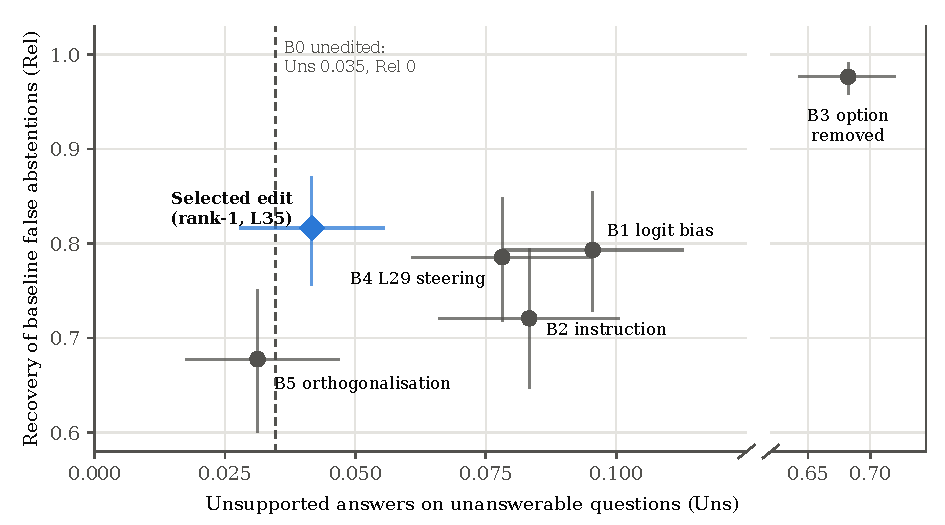
\includegraphics[width=\linewidth]{figures/fig2-tradeoff.pdf}
\caption{Recovery against unsupported answering on H for the selected edit and the five repair comparators. Up and to
the left is better. Bars are marginal 95\% bootstrap intervals for each rate, computed after confirmation from the
stored per-row outputs (\cref{app:figdata}). They are descriptive. The confirmatory comparisons in \cref{tab:h} use
paired differences and Holm correction, so overlapping marginal intervals do not imply that a comparison failed, and
separated ones do not imply that it passed. The dashed line marks the unedited model's unsupported-answer rate; its
recovery is 0 by definition. The horizontal axis is broken to show B3.}
\label{fig:tradeoff}
\end{figure}

\paragraph{Logit bias: inconclusive.}
The comparison with B1 is the most informative result in the study, because B1 is the simplest intervention that
targets the output directly. The point estimates favour the edit: recovery 0.816 against 0.793, and unsupported
answers 0.042 against 0.095. The difference in unsupported answers is clear (edit minus B1: $-0.054$, 95\% CI
$-0.069$ to $-0.038$). The difference in recovery is not ($+0.023$, 95\% CI $-0.043$ to $+0.088$). O2 therefore
depends on whether the edit's recovery is at most 0.05 below B1's. That non-inferiority component gave $p = 0.015$,
which did not survive Holm correction (adjusted $p = 0.092$). Equivalence was not shown either: TOST gave $p = 0.21$
for recovery and $0.70$ for unsupported answering. The data do not show that the edit is better than logit bias, and
they do not show that the two are equivalent. B1 also has an advantage the trade-off tests do not score: it broke no
previously correct answers.

\paragraph{Option removal: not established.}
Removing the ``unknown'' option (B3) recovered almost every false abstention (0.977), but it answered 0.682 of
unanswerable questions. The edit recovered less ($-0.160$) and gave far fewer unsupported answers ($-0.641$). Neither
orientation passes: O1 fails because the edit recovers less, and O2 fails because the recovery loss exceeds the 0.05
margin. The frozen tests cannot rank two arms that sit at such different points of the trade-off. On utility, which
weighs both sides equally, B3 scored 0.130 against the edit's 0.435, but utility was not a pre-specified comparison
between arms.

\paragraph{False abstentions whose note names the city.}
In 232 of the 261 false abstentions on H, the unedited model's note names the gold city (by the frozen
answer-bearing rule). On this subset, the edit and B1 recovered at similar rates (0.864 and 0.881). This comparison
is descriptive and was not tested.

\subsection{Transfer to unseen cities}

T-city has 24 bases per task and uses cities that appear in no other split. It was read once and is a descriptive
check, not a second confirmation. The results resemble those on H. Utility was 0.422 against 0.303 for the unedited
model, recovery 0.817, unsupported answering 0.062 against 0.059, damage 0.031 and counterfactual following 0.912.
Comparator utilities fell in the same order as on H: B4 0.415, B1 0.412, B5 0.409, B2 0.397, B3 0.107. T-city
changes only the answer vocabulary. It does not test new tasks or reworded instructions.

The edit's selection-split results were also close to its confirmation results (utility 0.429 on S and 0.435 on H;
counterfactual following 0.910 and 0.917). We report this consistency as description, not as extra evidence, because
S was used to select the edit.
